\section{系统实现与测试}

\subsection{开发平台和工具选择}

\paragraph{一、测试目标}

本阶段对“重庆邮电大学智慧访客预约与出入校管理系统”进行阶段性系统测试，目标是验证数据库脚本、后端服务、前端页面、登录认证、角色权限、访客预约审批、门岗核验、出入校登记、统计报表、自动截图和报告生成能力是否满足数据库原理课程设计要求。

\paragraph{二、测试环境}

\begin{longtable}{p{0.47\textwidth}p{0.47\textwidth}}
\toprule
项目 & 环境 \\
\midrule
操作系统 & Windows 11 \\
数据库 & MySQL Server 8.4，兼容 MySQL 8 语法 \\
后端 & JDK 17，Spring Boot 3，MyBatis Plus，JWT \\
构建工具 & Apache Maven 3.9.9 \\
前端 & Node.js v24.17.0，npm 11.13.0，Vue 3，Vite，Element Plus，ECharts \\
自动截图 & Playwright，系统 Chrome 兜底 \\
报告生成 & Python 3.12，python-docx \\
\bottomrule
\end{longtable}


\paragraph{三、测试范围}

测试范围覆盖数据库初始化、后端启动、前端启动、登录认证、RBAC 权限、访客预约、黑名单检查、被访人确认、部门审批、通行码生成、门岗核验、入校登记、离校登记、超时未离校、统计报表、自动截图和报告生成。

\paragraph{四、执行结果概览}

\begin{longtable}{p{0.23\textwidth}p{0.23\textwidth}p{0.23\textwidth}p{0.23\textwidth}}
\toprule
测试项 & 验证方式 & 实际结果 & 结论 \\
\midrule
数据库初始化 & `bash scripts/init\_database.sh` & 数据库 `cqupt\_visitor\_system` 重建成功 & 通过 \\
数据规模检查 & 查询核心表数量 & `sys\_user=13`、`visit\_apply=24`、`access\_record=13`、`blacklist=4`、`operation\_log=20` & 通过 \\
后端构建 & `mvn -DskipTests package` & 生成 `target/cqupt-visitor-backend-0.1.0.jar` & 通过 \\
前端构建 & `npm run build` & Vite 构建成功，仅存在 chunk 体积提示 & 通过 \\
自动截图 & `bash scripts/run\_all.sh` & 自动启动服务、登录角色、生成 19 张截图和 manifest & 通过 \\
端口清理 & `run\_all.sh` 结束后检查 8080/5173 & 无残留监听进程 & 通过 \\
报告生成 & `python scripts/generate\_report.py` & 自动生成 Markdown 和 Word 报告 & 通过 \\
\bottomrule
\end{longtable}


\paragraph{五、问题与修复概况}

测试过程中发现并修复了 Maven 缺失、Playwright Chromium 下载慢、后端启动脚本使用 `spring-boot:run` 找不到主类、一键脚本退出后残留服务进程、数据库缺少最新演示数据等问题。详细记录见根目录 `bug\_fix\_log.md`。

\paragraph{六、结论}

系统当前具备完整的数据库初始化、后端构建、前端构建、核心页面展示、自动截图和报告生成能力。核心业务流程已通过演示数据和自动化截图验证，适合作为课程设计报告和答辩演示的基础版本。后续可继续补充更细粒度的接口自动化测试和单元测试。

\subsection{系统测试}

\begin{longtable}{p{0.09\textwidth}p{0.09\textwidth}p{0.09\textwidth}p{0.09\textwidth}p{0.09\textwidth}p{0.09\textwidth}p{0.09\textwidth}p{0.09\textwidth}p{0.09\textwidth}p{0.09\textwidth}}
\toprule
测试编号 & 测试名称 & 测试目的 & 前置条件 & 输入数据 & 操作步骤 & 预期结果 & 实际结果 & 是否通过 & 备注 \\
\midrule
TC-001 & 数据库初始化测试 & 验证建库、建表、初始化数据脚本可重复执行 & MySQL 已启动 & `scripts/init\_database.sh` & 在 `project` 目录执行初始化脚本 & 成功创建 `cqupt\_visitor\_system` 并插入演示数据 & 数据库初始化成功，核心表数据量正常 & 通过 & 会重建课程设计演示库 \\
TC-002 & 数据库核心表数量测试 & 验证演示数据覆盖核心页面 & 已执行初始化脚本 & 查询 `sys\_user`、`visit\_apply`、`access\_record` 等 & 执行表数量 SQL & 用户、预约、出入校、黑名单、日志均有数据 & `sys\_user=13`、`visit\_apply=24`、`access\_record=13`、`blacklist=4`、`operation\_log=20` & 通过 & 支撑报表和截图 \\
TC-003 & 后端构建测试 & 验证 Spring Boot 项目可编译打包 & JDK 17、Maven 可用 & `mvn -DskipTests package` & 在 `backend` 目录执行命令 & 生成可运行 jar & 构建成功并生成后端 jar & 通过 & 测试跳过单元测试 \\
TC-004 & 前端构建测试 & 验证 Vue 3 项目可构建 & Node/npm 已安装 & `npm run build` & 在 `frontend` 目录执行命令 & Vite 构建成功 & 构建成功，有 chunk 体积提示但不影响运行 & 通过 & 可后续做代码分包优化 \\
TC-005 & 登录测试 & 验证默认账号可登录并返回 Token & 后端和前端运行 & `admin / 123456` & 打开登录页输入账号密码 & 登录成功进入首页驾驶舱 & 自动截图流程成功登录并进入 `/dashboard` & 通过 & JWT 自动写入请求头 \\
TC-006 & 权限菜单测试 & 验证不同角色菜单范围正确 & 已登录不同角色 & `admin`、`teacher01`、`approver01`、`guard01`、`manager01` & 自动截图脚本切换账号访问页面 & 各角色只能看到授权菜单 & 19 个页面按角色成功访问并截图 & 通过 & 访客、被访人、审批、门岗、校级管理均覆盖 \\
TC-007 & 访客预约申请页面测试 & 验证预约表单可展示完整字段 & 访客账号登录 & `visitor01 / 123456` & 访问 `/visit/apply` & 表单包含访客、被访人、访问时间、事由、车辆等字段 & `03\_visitor\_apply.png` 生成成功 & 通过 & 页面字段与后端 DTO 对齐 \\
TC-008 & 我的预约查询测试 & 验证访客可查看自己的预约状态 & 访客账号登录 & `visitor01` & 访问 `/visit/mine` & 显示我的预约列表和状态标签 & `04\_my\_apply.png` 生成成功 & 通过 & 覆盖待确认、审批通过等状态 \\
TC-009 & 黑名单检查测试 & 验证黑名单数据可展示并用于业务拦截 & 管理员账号登录 & 黑名单手机号/证件号 & 访问黑名单页并检查数据 & 黑名单访客被标记或拦截 & `12\_blacklist.png` 生成成功，库中 `blacklist=4` & 通过 & 业务拦截逻辑在预约服务中实现 \\
TC-010 & 被访人确认测试 & 验证被访人只能处理本人相关预约 & 被访人账号登录 & `teacher01` & 访问 `/approval/host` & 显示待确认预约，可确认或拒绝 & `05\_host\_confirm.png` 生成成功 & 通过 & 数据范围按当前用户过滤 \\
TC-011 & 部门审批测试 & 验证部门审批人员可处理本部门预约 & 审批账号登录 & `approver01` & 访问 `/approval/department` & 显示本部门待审批预约 & `06\_department\_approval.png` 生成成功 & 通过 & 通过后生成通行凭证 \\
TC-012 & 通行码生成测试 & 验证审批通过后可查询通行凭证 & 已有审批通过预约 & `pass\_code` 表 & 访问通行凭证相关页面或接口 & 存在有效期内通行码 & 初始化数据含多条 `pass\_code`，截图流程正常 & 通过 & 拒绝/取消预约不能生成通行码 \\
TC-013 & 门岗核验测试 & 验证门岗可按通行码、手机号或预约号核验 & 门岗账号登录 & `guard01` & 访问 `/gate/verify` & 显示核验表单和结果区 & `07\_gate\_check.png` 生成成功 & 通过 & 会检查黑名单、审批状态、访问时间 \\
TC-014 & 入校登记测试 & 验证核验通过后可记录入校信息 & 门岗账号登录 & 已审批通过预约 & 访问 `/access/entry` & 可填写校门、安保人员、入校时间 & `08\_enter\_register.png` 生成成功 & 通过 & 访问状态更新为已入校 \\
TC-015 & 离校登记测试 & 验证已入校访客可登记离校且不可重复离校 & 门岗账号登录 & 已入校记录 & 访问 `/access/exit` & 可完成离校登记 & `09\_leave\_register.png` 生成成功 & 通过 & 服务层限制重复离校 \\
TC-016 & 当前在校访客测试 & 验证可查询已入校未离校访客 & 门岗账号登录 & `access\_status=ENTERED` & 访问 `/access/current` & 展示当前在校访客列表 & `10\_current\_visitor.png` 生成成功 & 通过 & 后端支持访问状态过滤 \\
TC-017 & 超时未离校测试 & 验证超时未离校访客可查询和标记 & 门岗账号登录 & `access\_status=OVERTIME` & 访问 `/access/overtime` & 展示超时访客 & `11\_overtime\_visitor.png` 生成成功 & 通过 & 初始化数据含超时记录 \\
TC-018 & 统计报表测试 & 验证统计接口和图表可展示 & 校级管理账号登录 & `manager01` & 访问 `/reports` & 显示趋势、部门排行、校门通行、审批通过率 & `14\_statistics.png` 生成成功 & 通过 & 统计接口 `/api/statistics/**` 已加入鉴权 \\
TC-019 & 自动截图测试 & 验证截图脚本可重复执行 & 前后端、数据库可运行 & `bash scripts/run\_all.sh` & 执行一键脚本 & 生成固定文件名截图和 manifest & 19 张 PNG 和 manifest 全部 `SUCCESS` & 通过 & 使用系统 Chrome 兜底 \\
TC-020 & 报告生成测试 & 验证报告生成器可读取文档、SQL、截图并导出报告 & 已生成测试文档和截图 & `python scripts/generate\_report.py` & 执行报告脚本 & 生成 Markdown 和 Word 报告 & Markdown/Word 均生成成功 & 通过 & Word 使用 python-docx 导出 \\
\bottomrule
\end{longtable}


\subsection{代表性运行界面}

以下截图由 Playwright 自动访问系统核心页面后生成，并同步到本 LaTeX 项目的 \texttt{figures/} 目录。每张图对应截图清单中的页面说明。

展示系统标题、登录表单、测试账号提示和校园蓝视觉风格。

\begin{figure}[H]

  \centering

  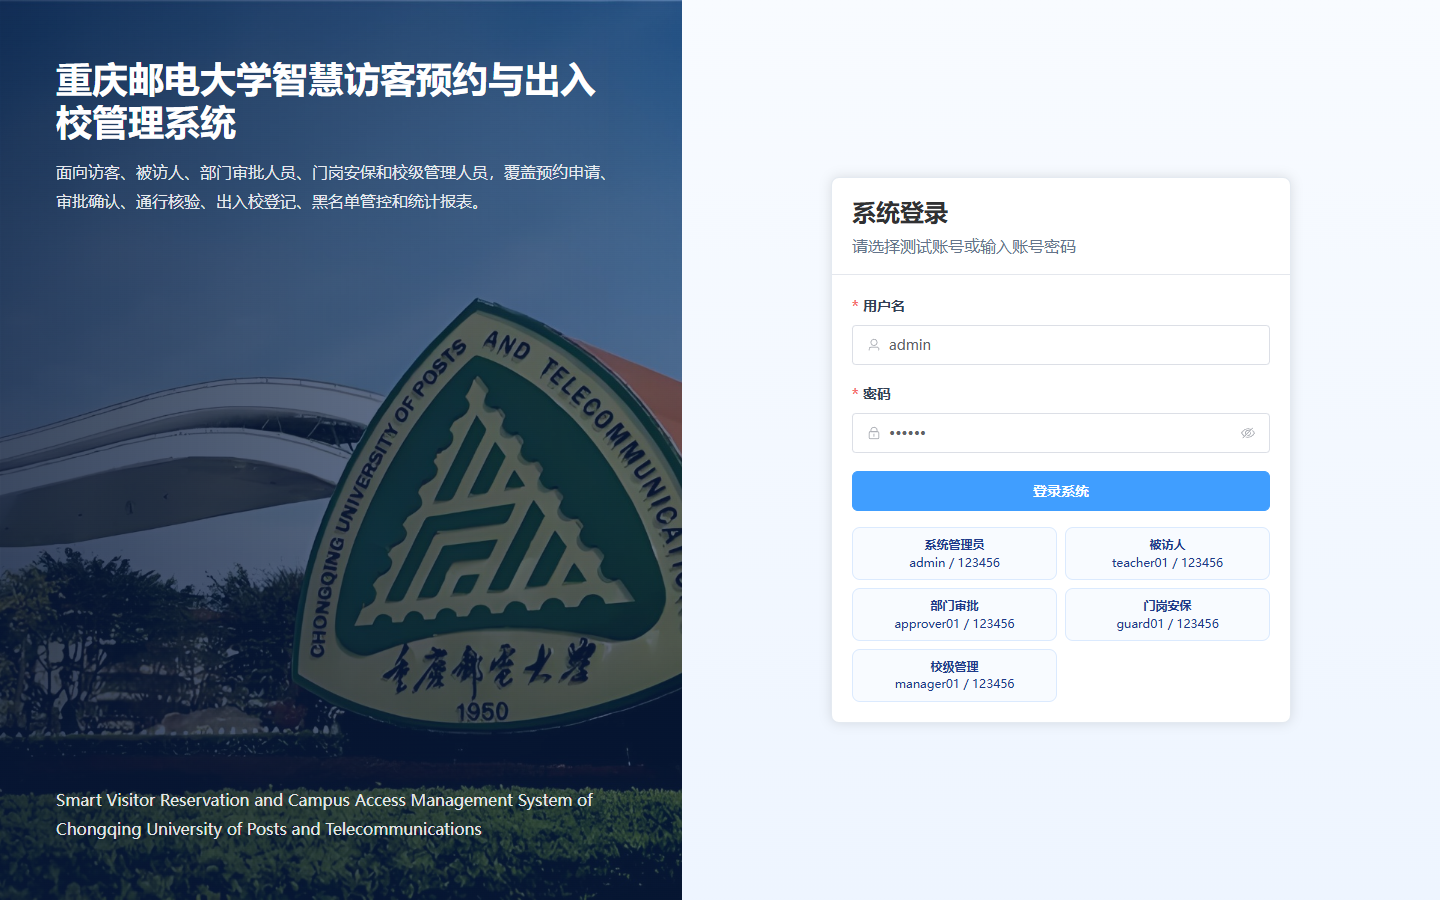
\includegraphics[width=0.92\textwidth]{figures/01_login.png}

  \caption{登录页}

\end{figure}

展示今日访客数、当前在校访客、超时未离校、部门访客排行、校门通行统计等核心指标。

\begin{figure}[H]

  \centering

  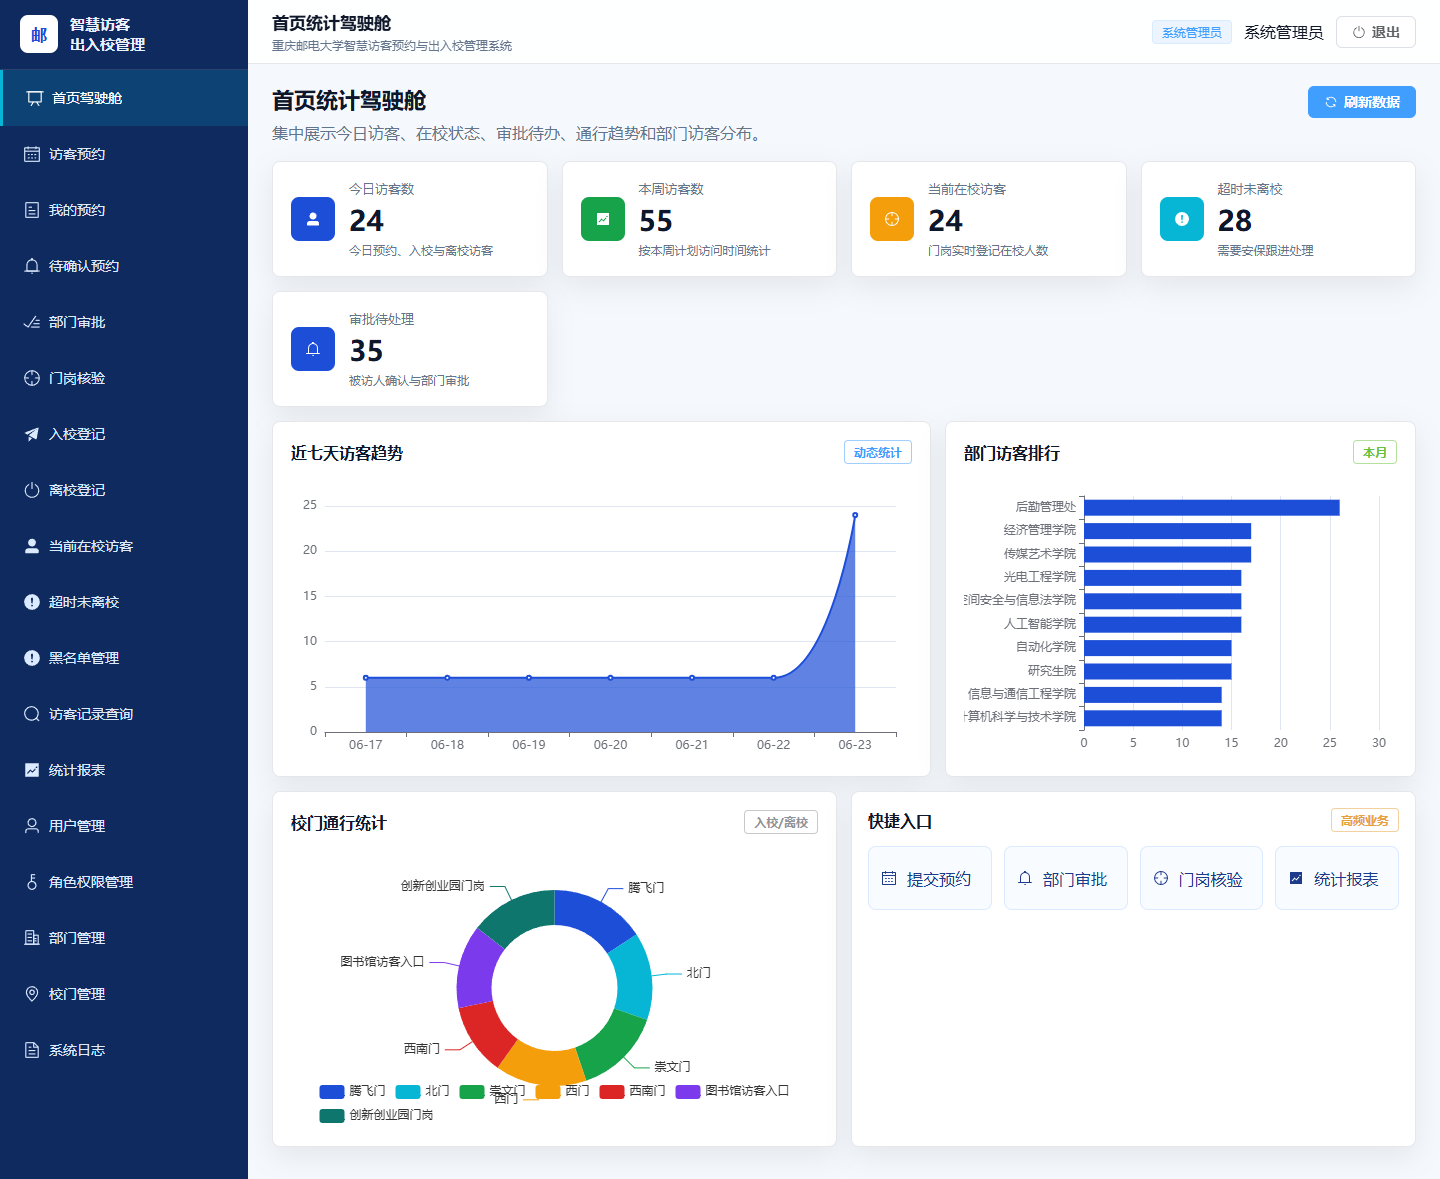
\includegraphics[width=0.92\textwidth]{figures/02_dashboard.png}

  \caption{首页统计驾驶舱}

\end{figure}

展示访客填写来访事由、被访人、访问时间、车辆和随行人员等预约申请信息。

\begin{figure}[H]

  \centering

  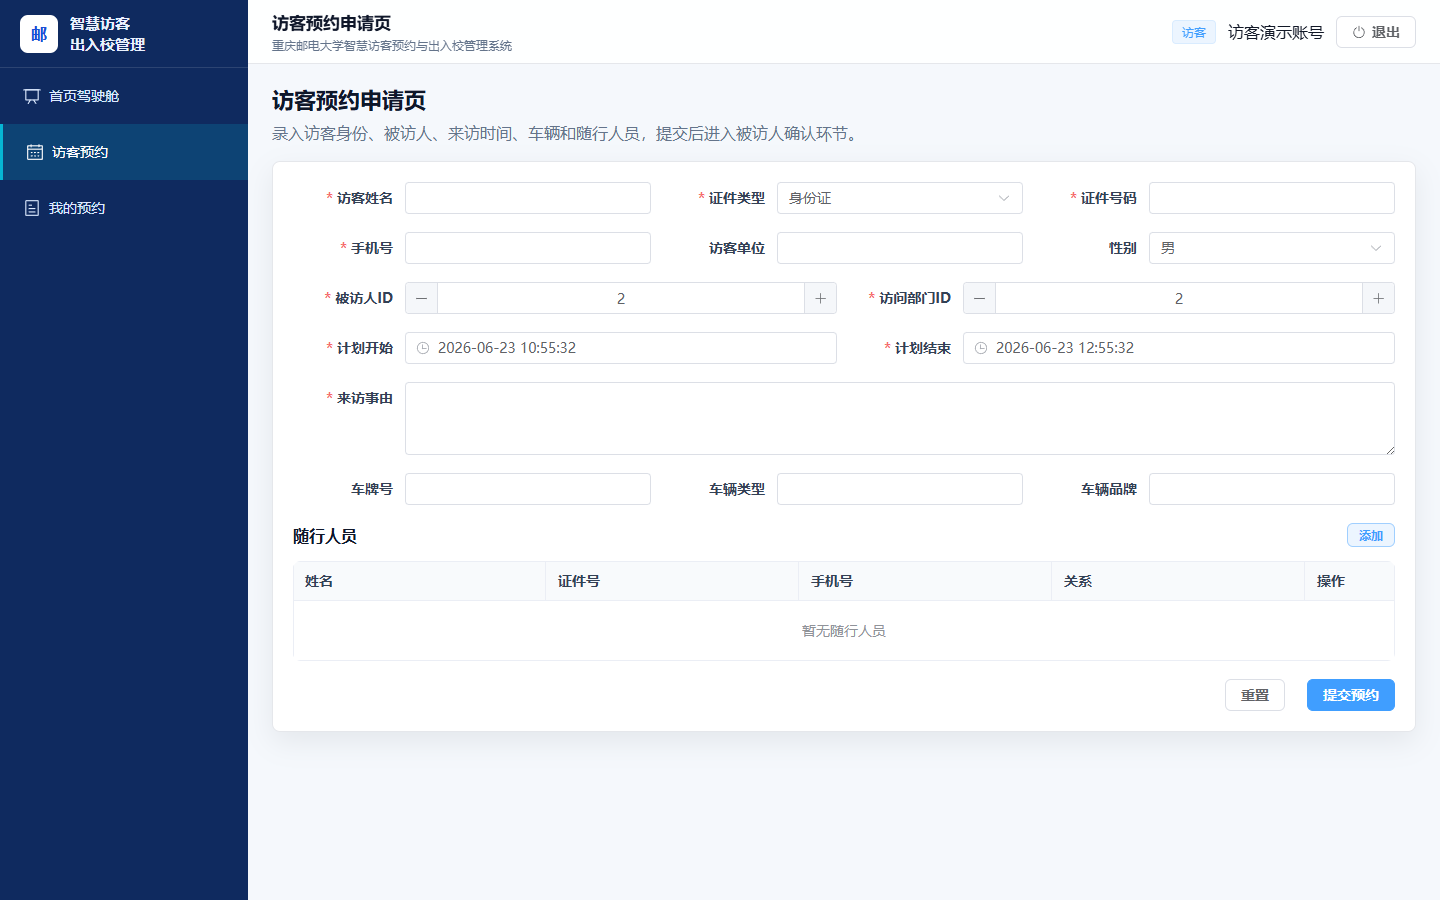
\includegraphics[width=0.92\textwidth]{figures/03_visitor_apply.png}

  \caption{访客预约申请页}

\end{figure}

展示预约记录、审批状态和访问状态，便于说明访客端状态查询功能。

\begin{figure}[H]

  \centering

  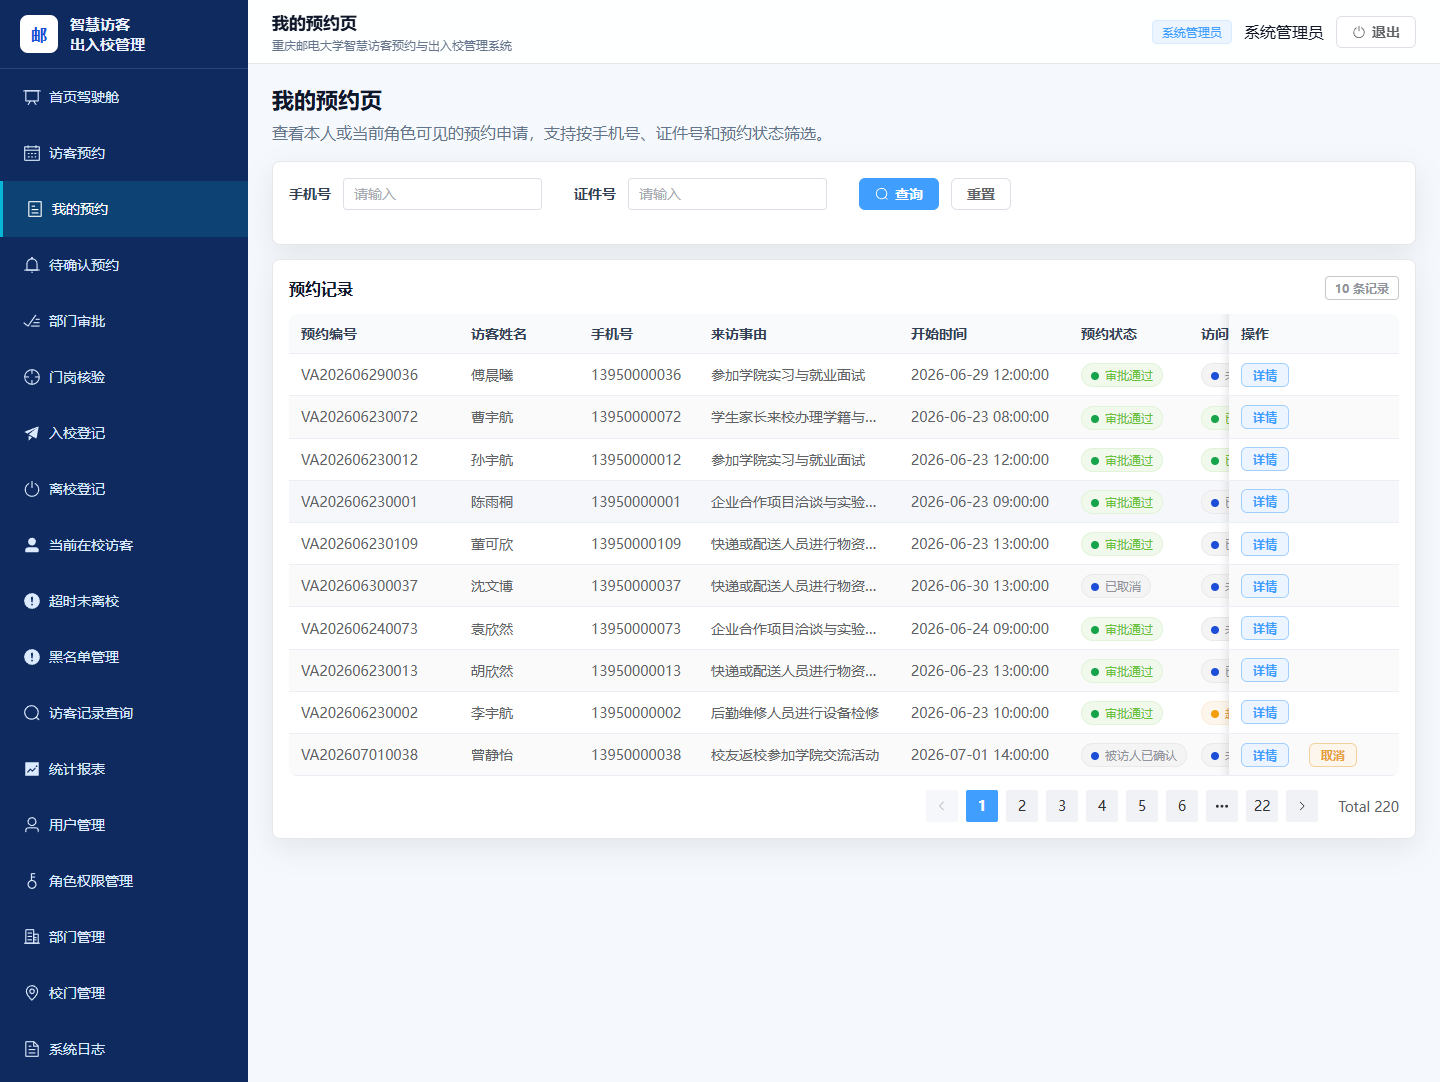
\includegraphics[width=0.92\textwidth]{figures/04_my_apply.png}

  \caption{我的预约页}

\end{figure}

展示被访人确认或拒绝预约申请的业务界面。

\begin{figure}[H]

  \centering

  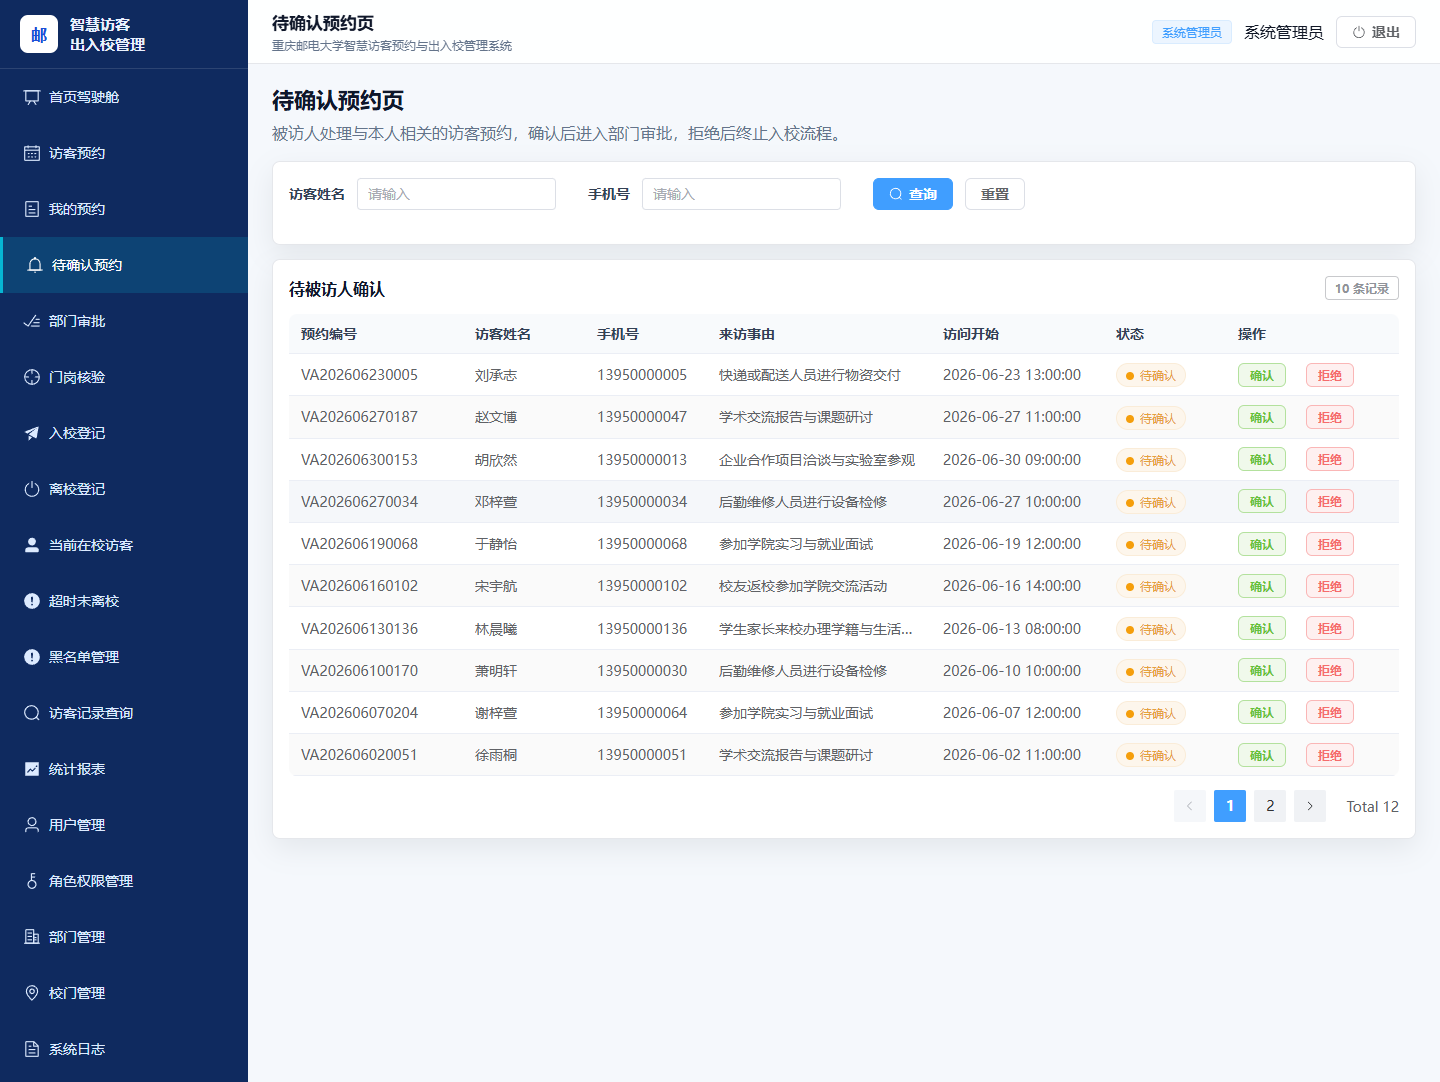
\includegraphics[width=0.92\textwidth]{figures/05_host_confirm.png}

  \caption{被访人待确认页}

\end{figure}

展示部门审批人员处理预约申请、填写审批意见和查看审批状态的功能。

\begin{figure}[H]

  \centering

  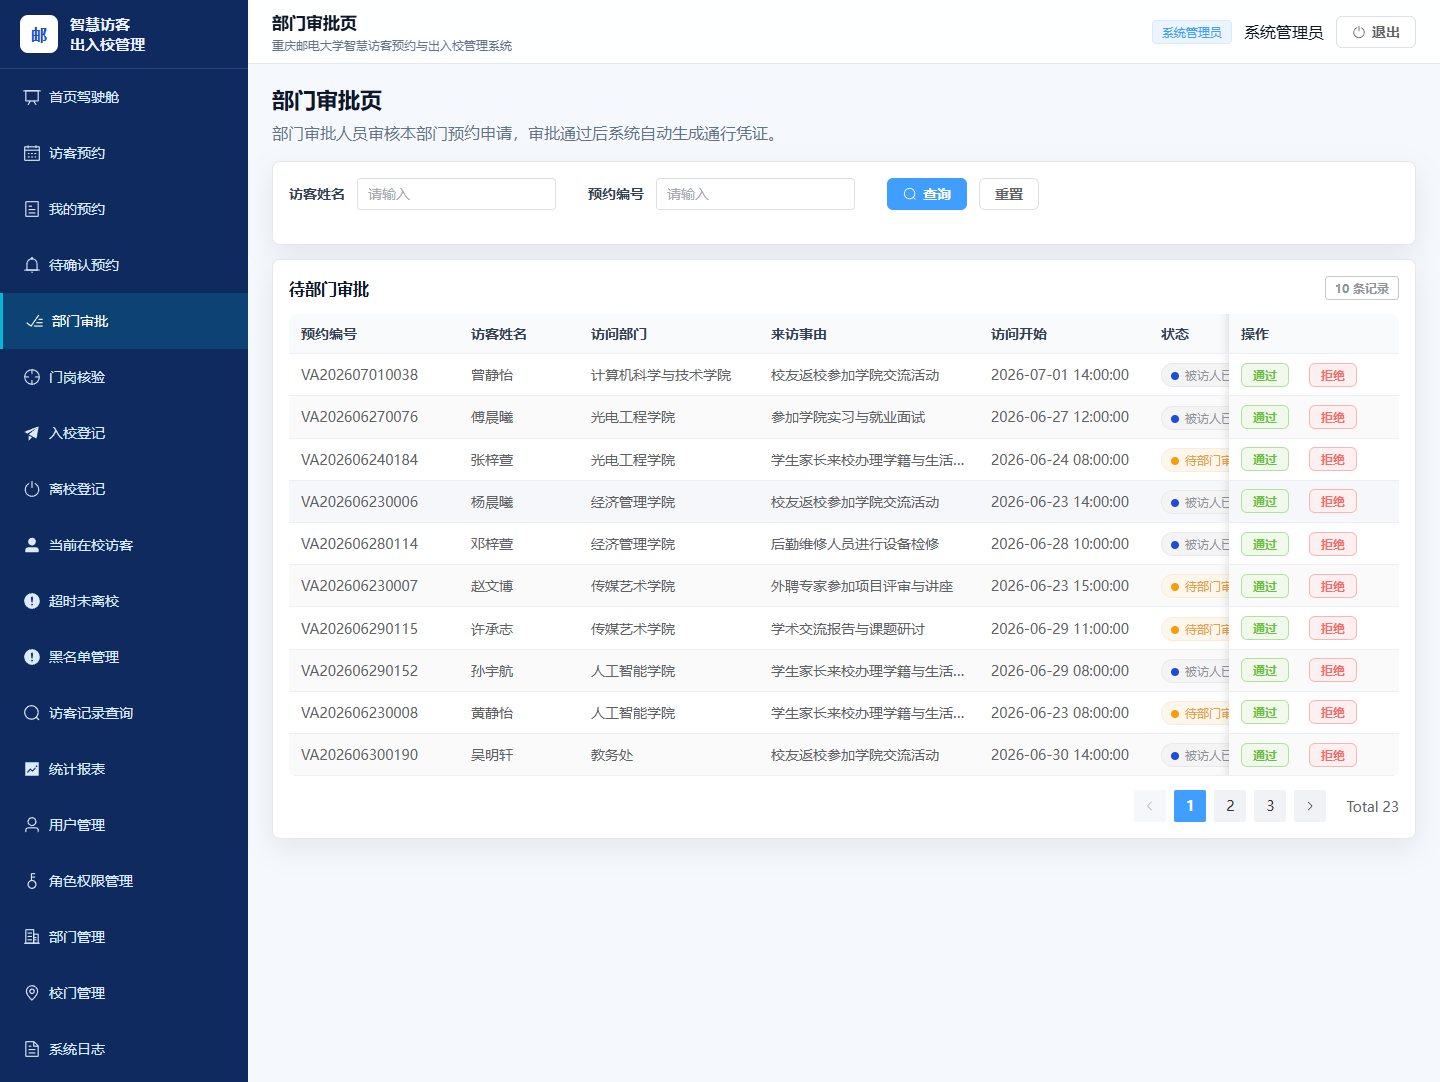
\includegraphics[width=0.92\textwidth]{figures/06_department_approval.png}

  \caption{部门审批页}

\end{figure}

展示门岗按预约编号、手机号、证件号或通行码进行访客核验的界面。

\begin{figure}[H]

  \centering

  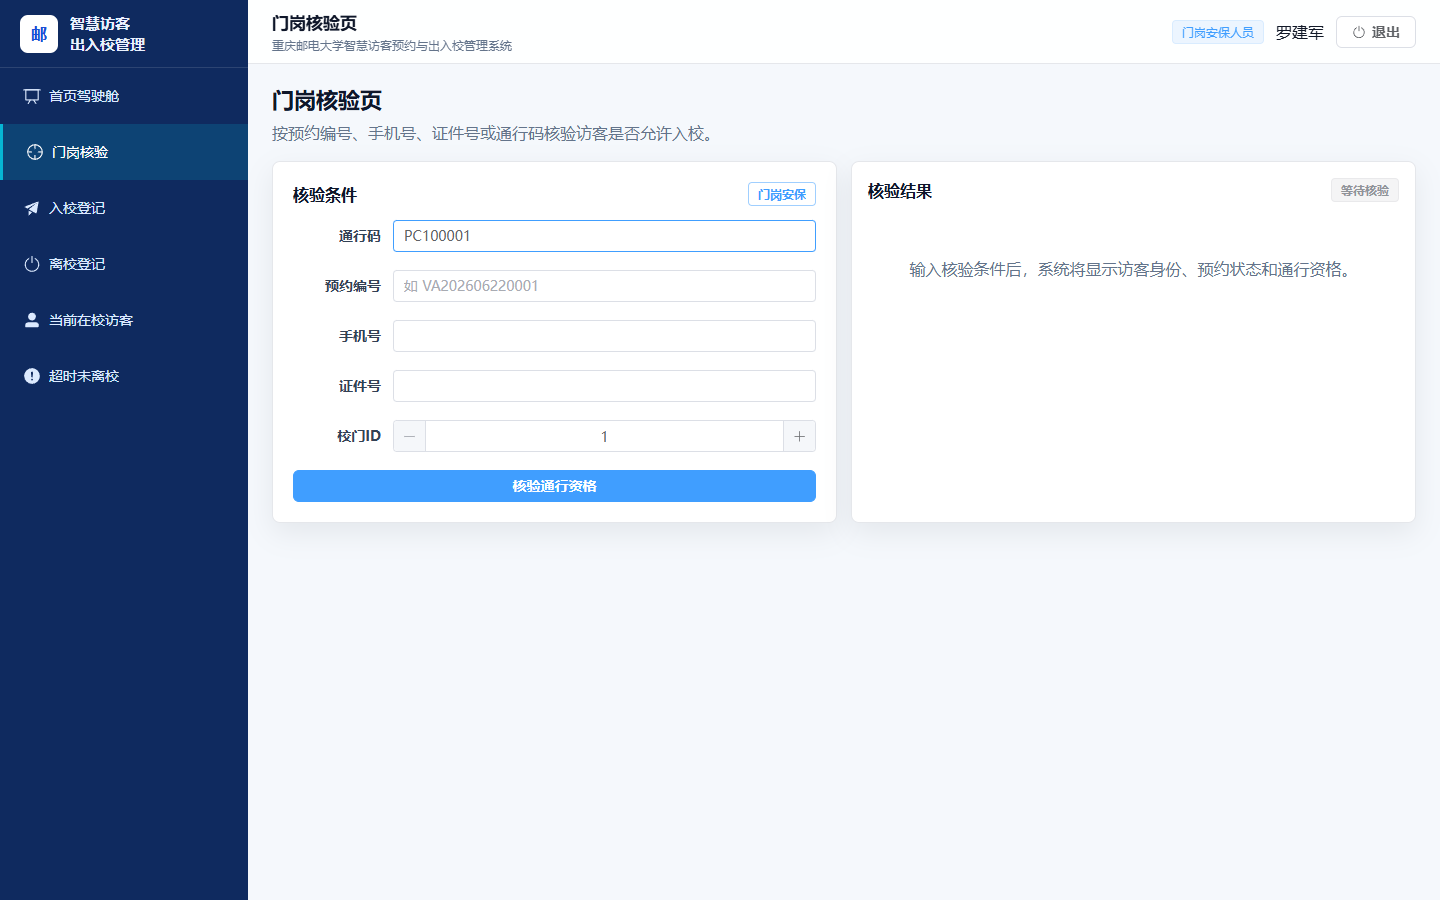
\includegraphics[width=0.92\textwidth]{figures/07_gate_check.png}

  \caption{门岗核验页}

\end{figure}

展示核验通过后记录入校时间、校门和安保人员的登记页面。

\begin{figure}[H]

  \centering

  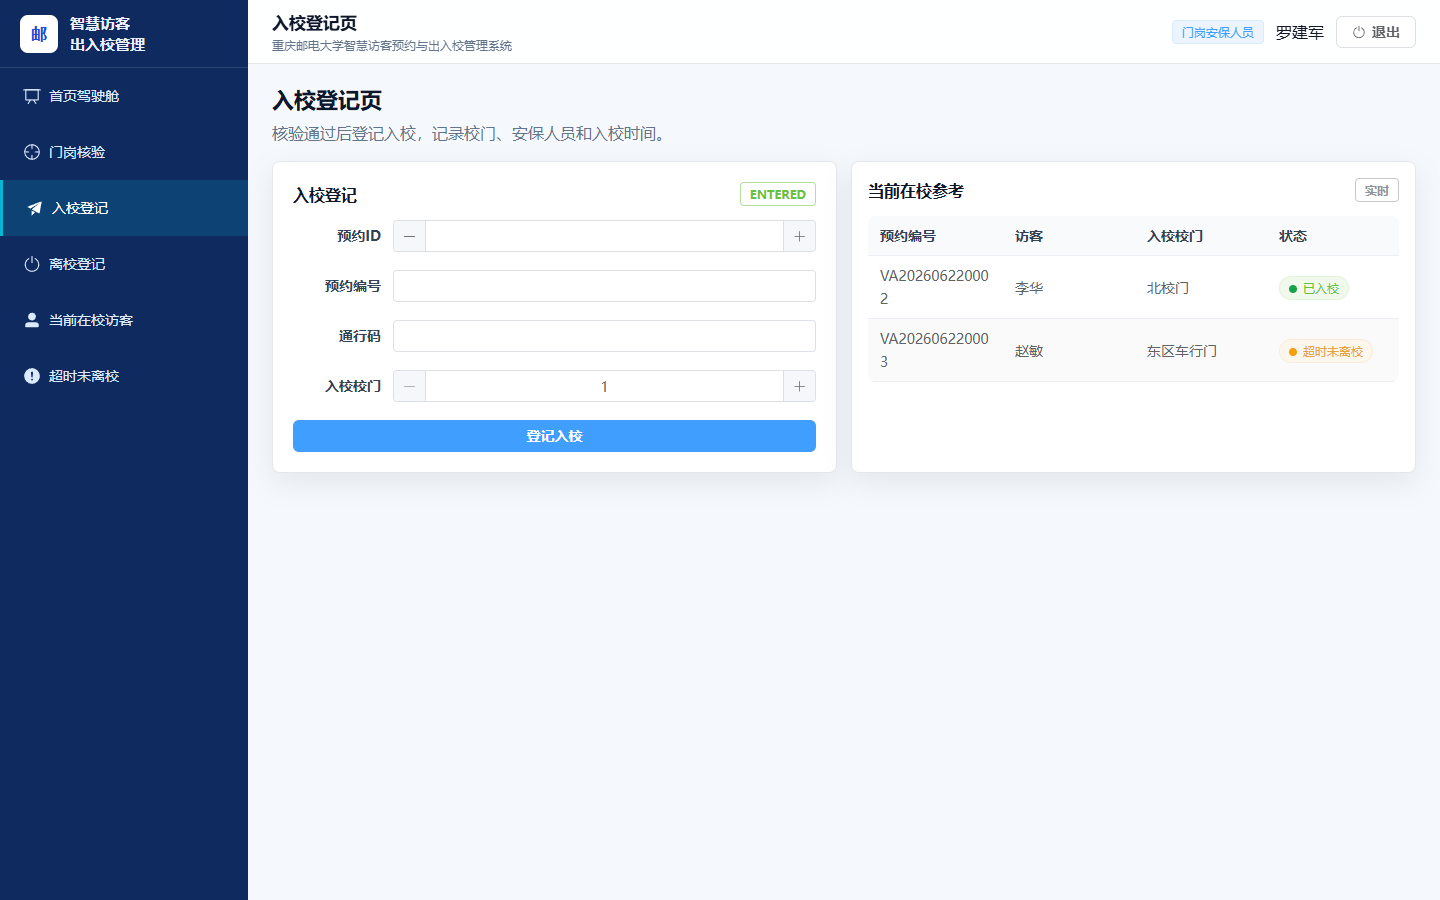
\includegraphics[width=0.92\textwidth]{figures/08_enter_register.png}

  \caption{入校登记页}

\end{figure}

展示已入校访客离校登记和访问状态更新功能。

\begin{figure}[H]

  \centering

  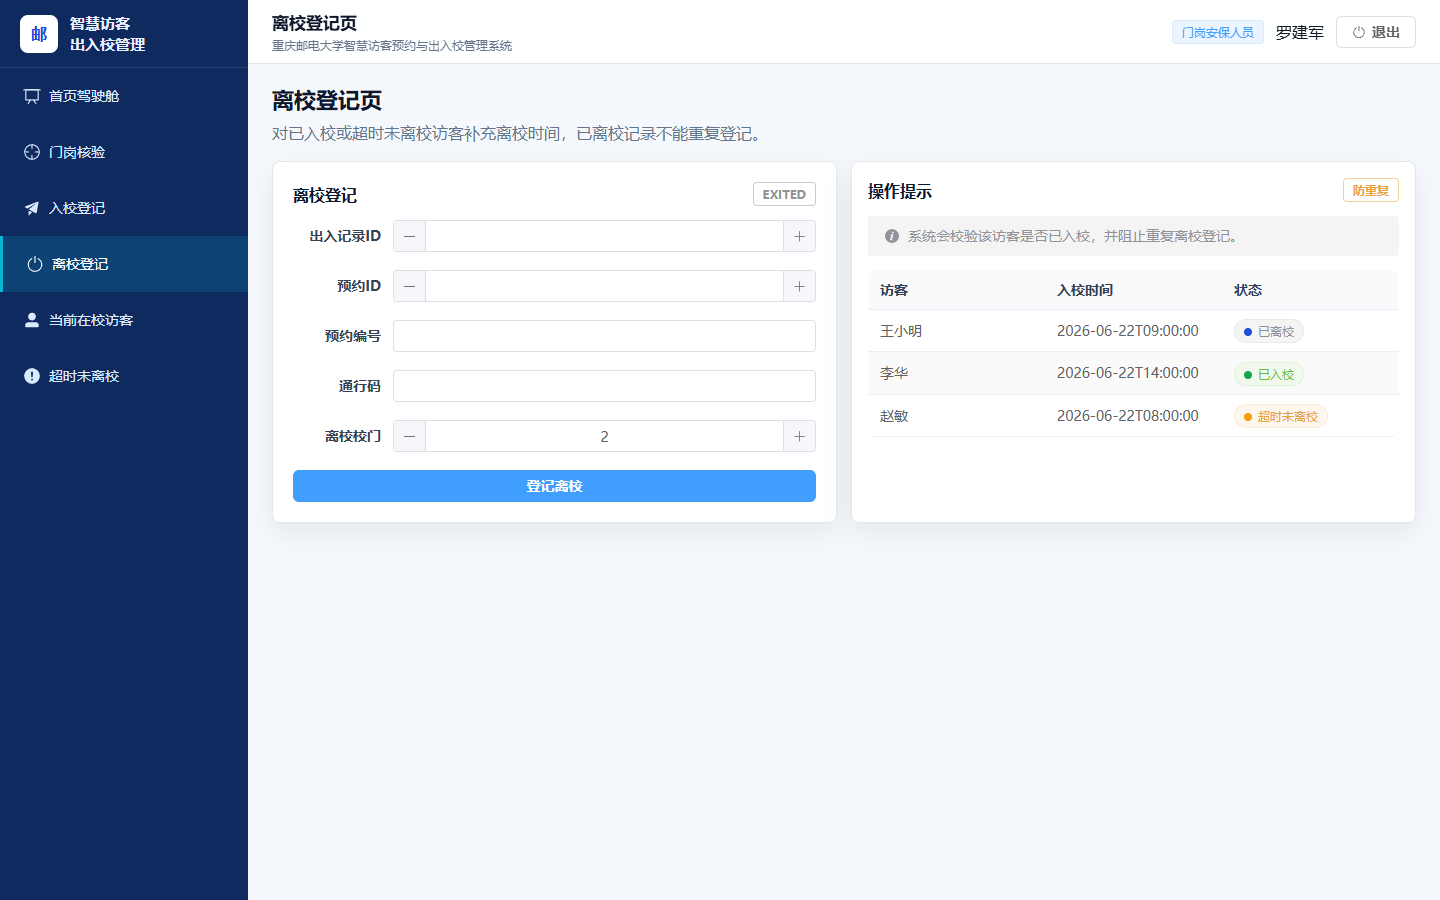
\includegraphics[width=0.92\textwidth]{figures/09_leave_register.png}

  \caption{离校登记页}

\end{figure}

展示当前已入校但尚未离校的访客列表。

\begin{figure}[H]

  \centering

  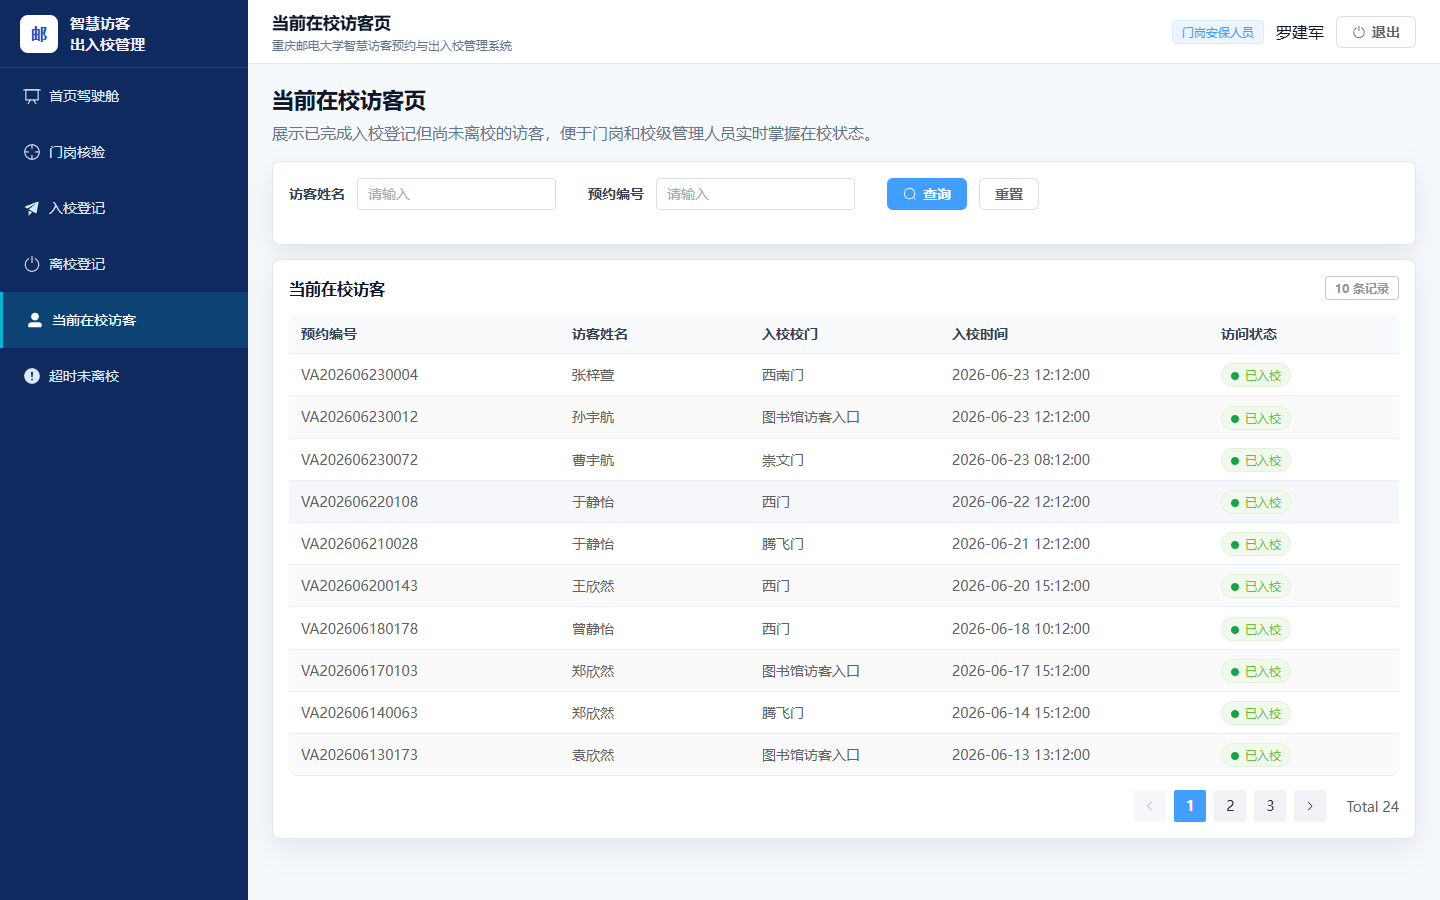
\includegraphics[width=0.92\textwidth]{figures/10_current_visitor.png}

  \caption{当前在校访客页}

\end{figure}

展示超过预计离校时间仍未离校的访客及风险提示。

\begin{figure}[H]

  \centering

  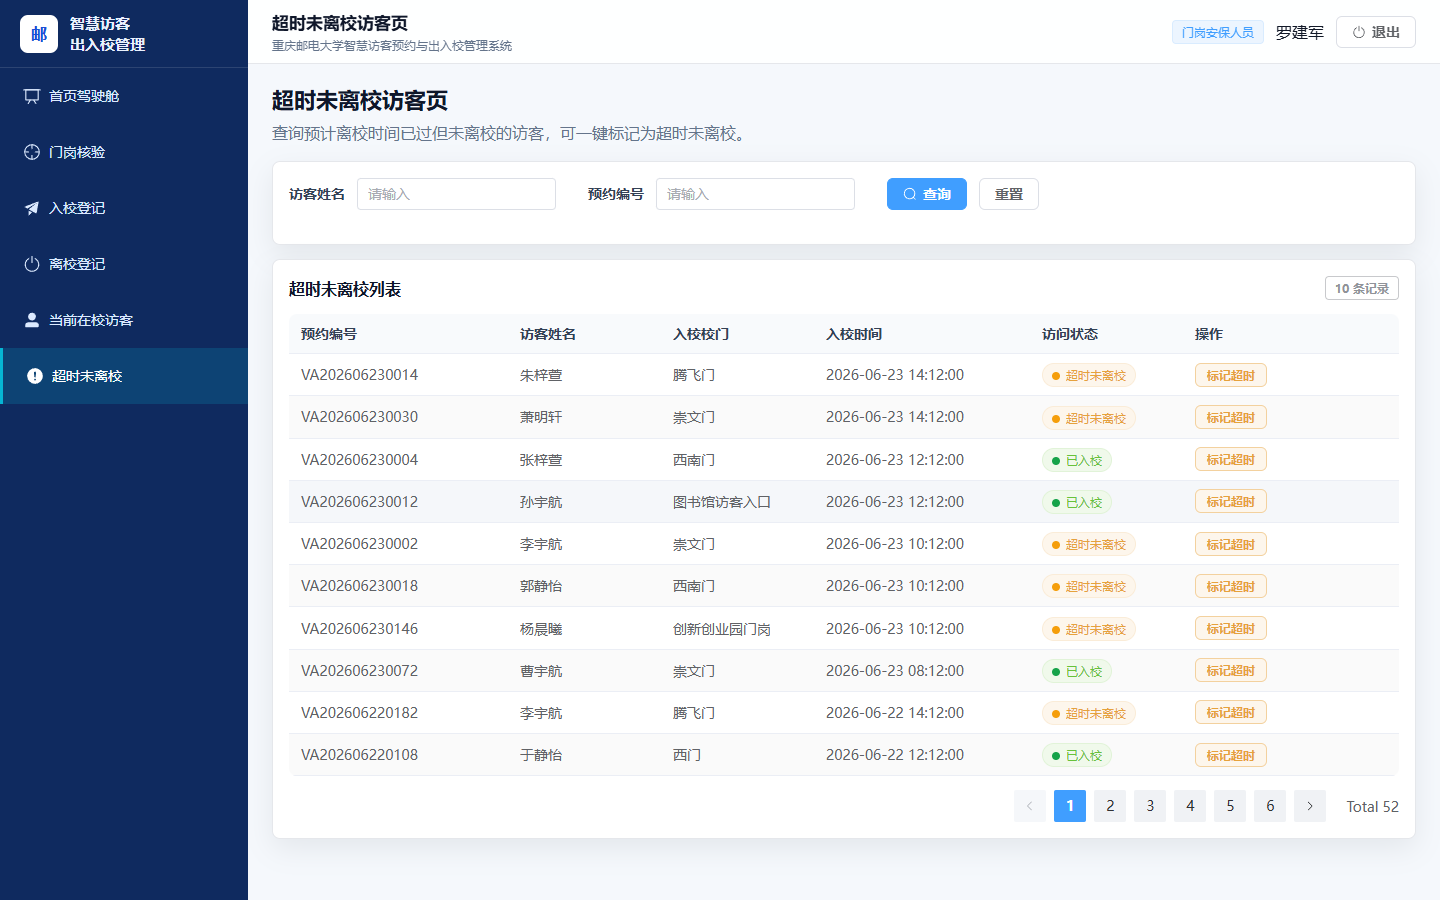
\includegraphics[width=0.92\textwidth]{figures/11_overtime_visitor.png}

  \caption{超时未离校访客页}

\end{figure}

展示身份异常、多次超时、虚假预约等风险访客黑名单管理。

\begin{figure}[H]

  \centering

  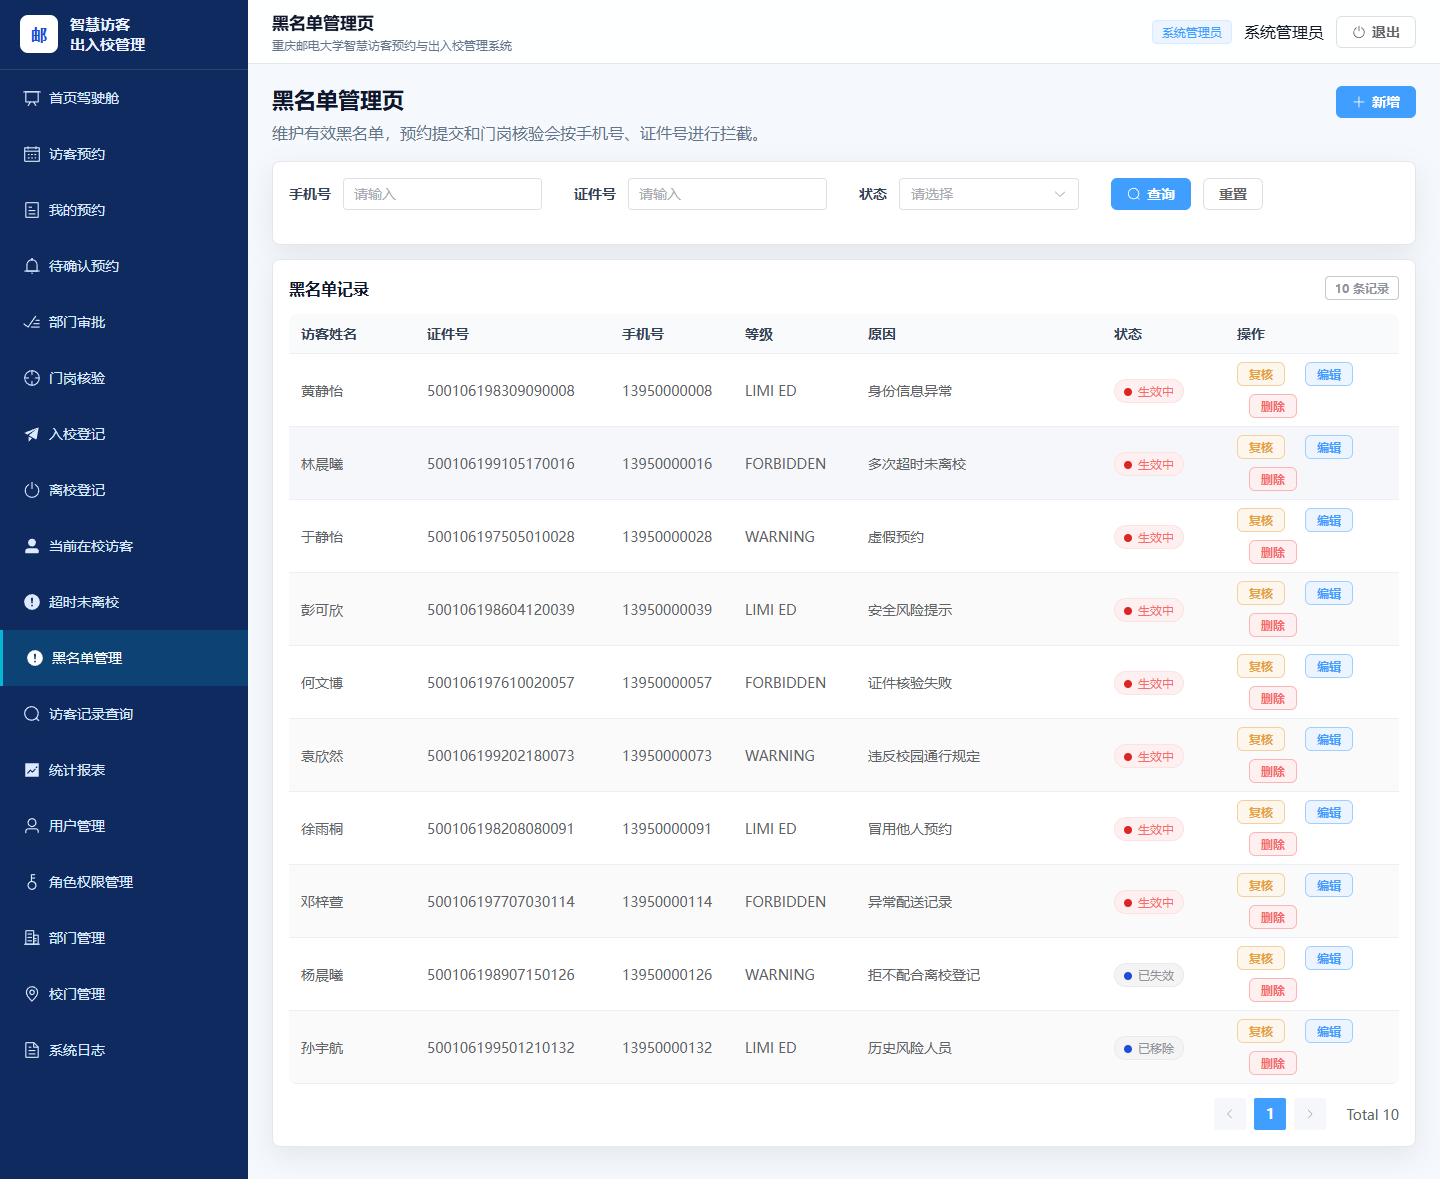
\includegraphics[width=0.92\textwidth]{figures/12_blacklist.png}

  \caption{黑名单管理页}

\end{figure}

展示按访客、部门、时间和状态查询全校访客记录的功能。

\begin{figure}[H]

  \centering

  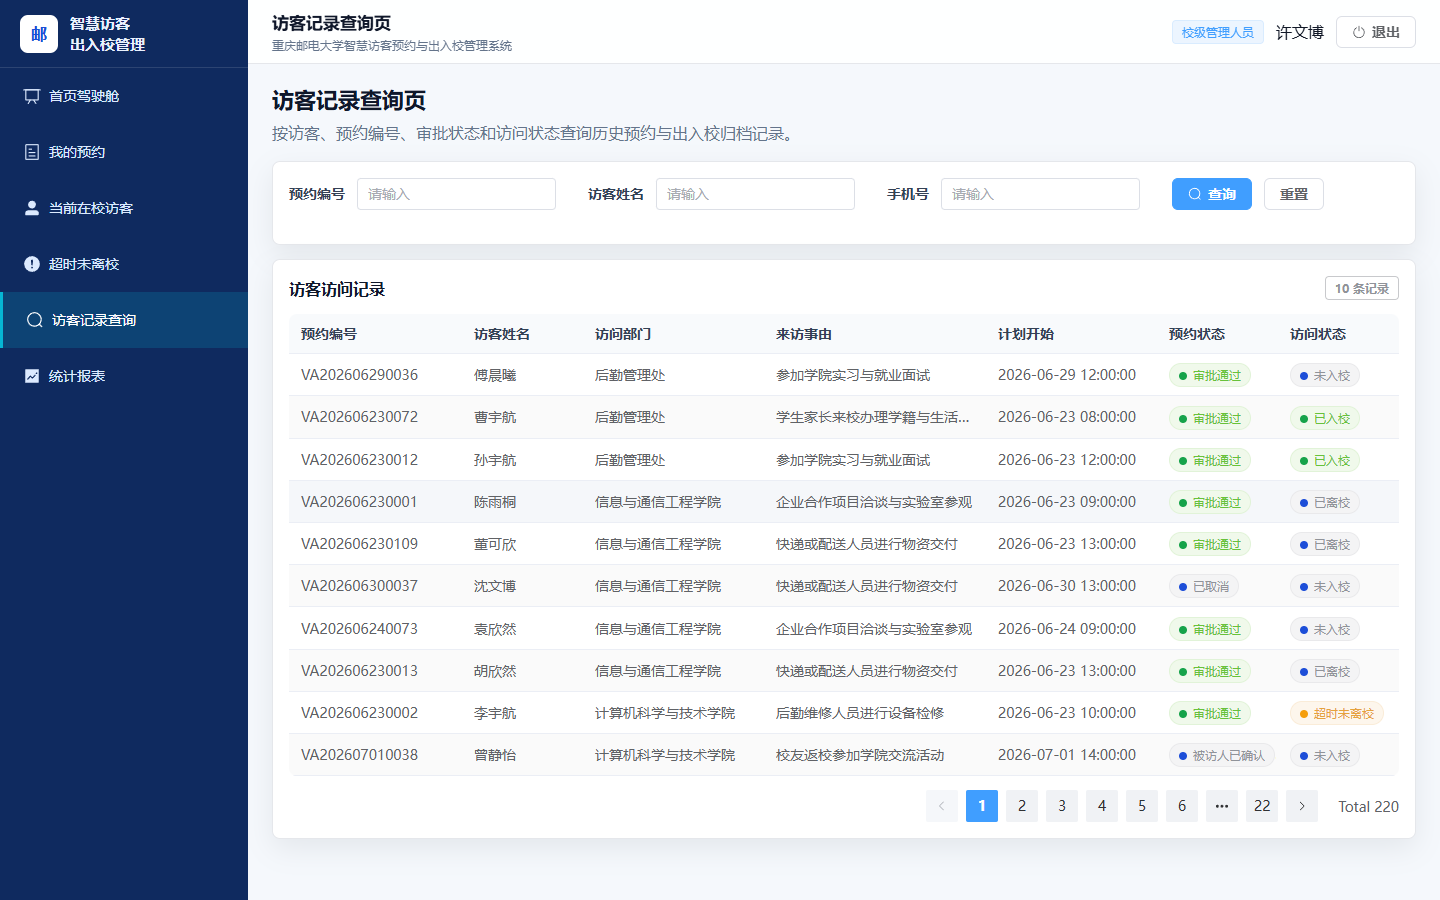
\includegraphics[width=0.92\textwidth]{figures/13_visit_record.png}

  \caption{访客记录查询页}

\end{figure}

展示近七天访客趋势、部门访客排行、校门通行统计、审批状态和黑名单风险等图表。

\begin{figure}[H]

  \centering

  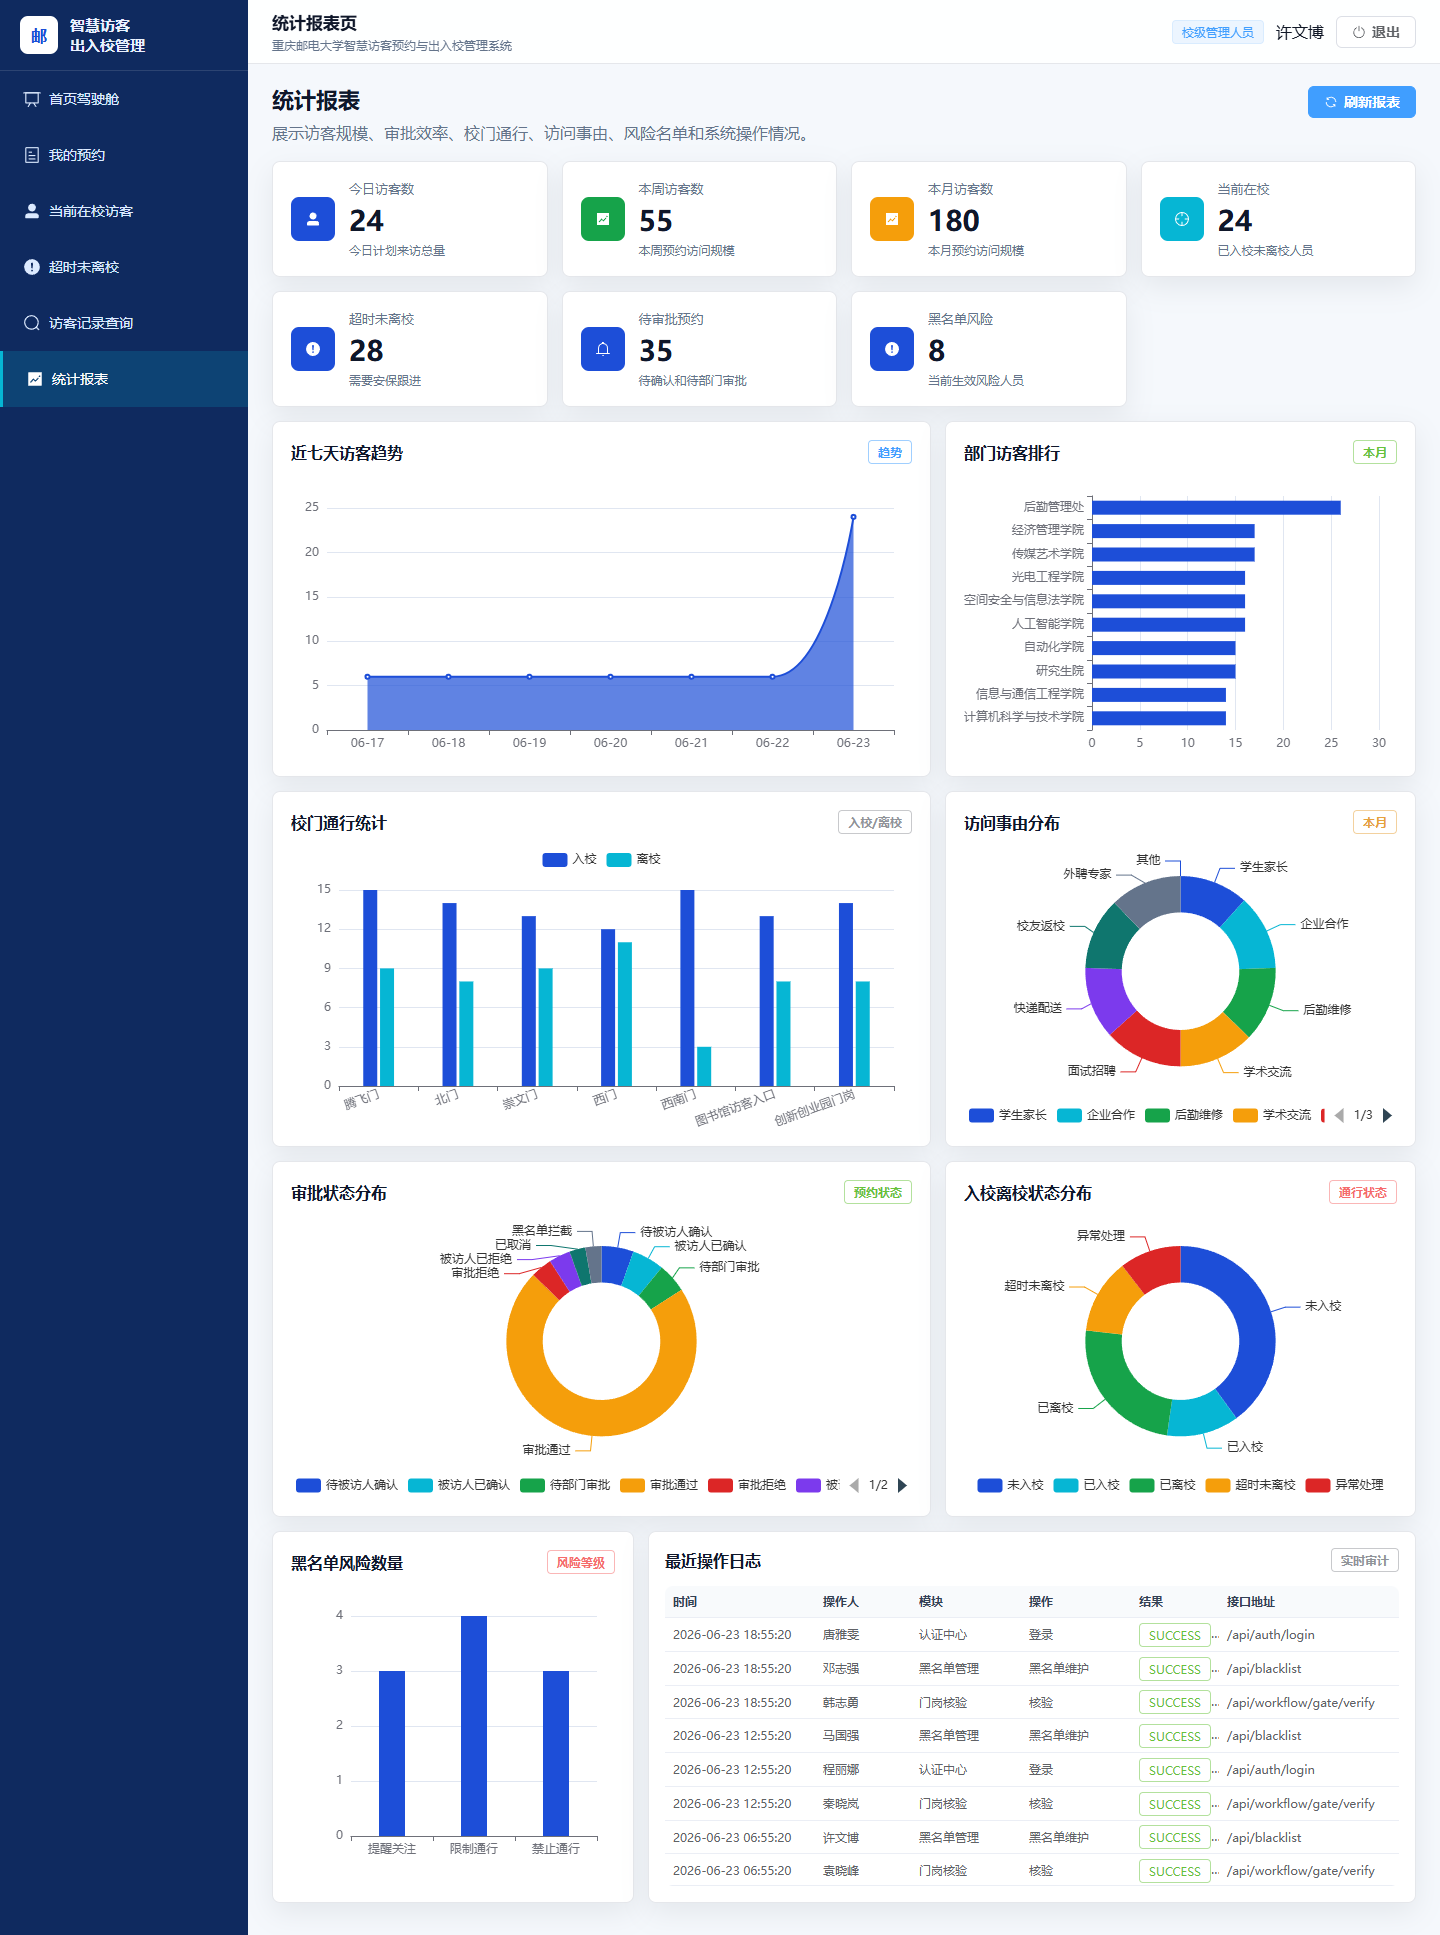
\includegraphics[width=0.92\textwidth]{figures/14_statistics.png}

  \caption{统计报表页}

\end{figure}

展示系统用户账号、角色类型、所属部门和账号状态管理。

\begin{figure}[H]

  \centering

  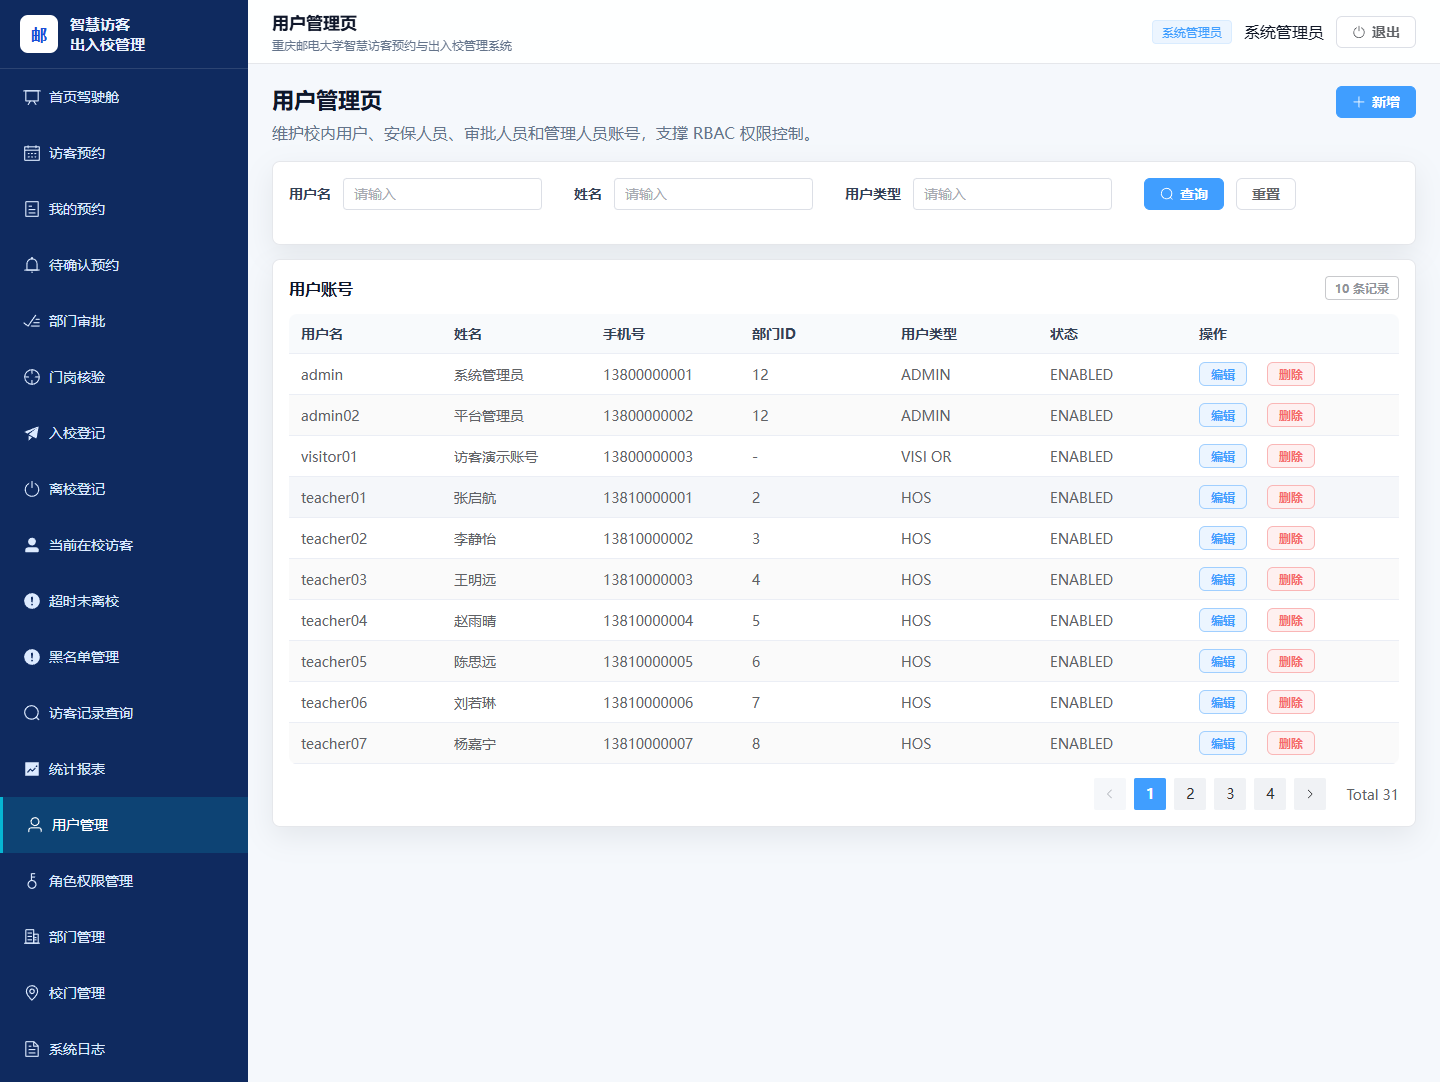
\includegraphics[width=0.92\textwidth]{figures/15_user_manage.png}

  \caption{用户管理页}

\end{figure}

展示系统角色和权限配置，支撑 RBAC 权限控制。

\begin{figure}[H]

  \centering

  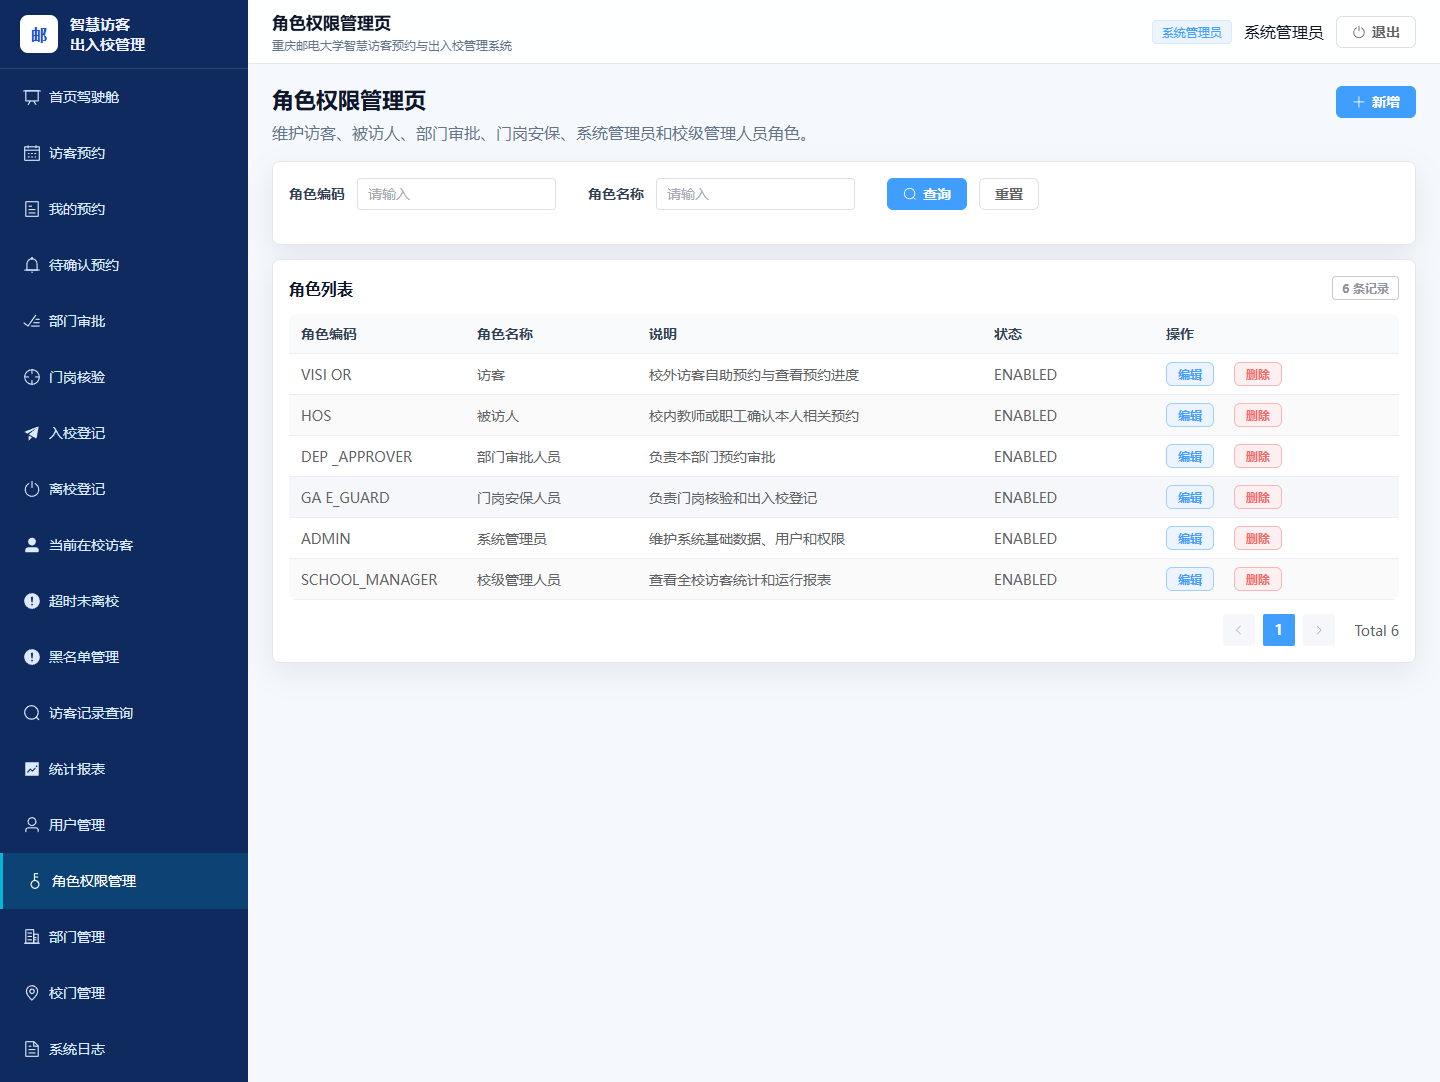
\includegraphics[width=0.92\textwidth]{figures/16_role_permission.png}

  \caption{角色权限管理页}

\end{figure}

展示学院、职能部门等组织结构基础数据维护。

\begin{figure}[H]

  \centering

  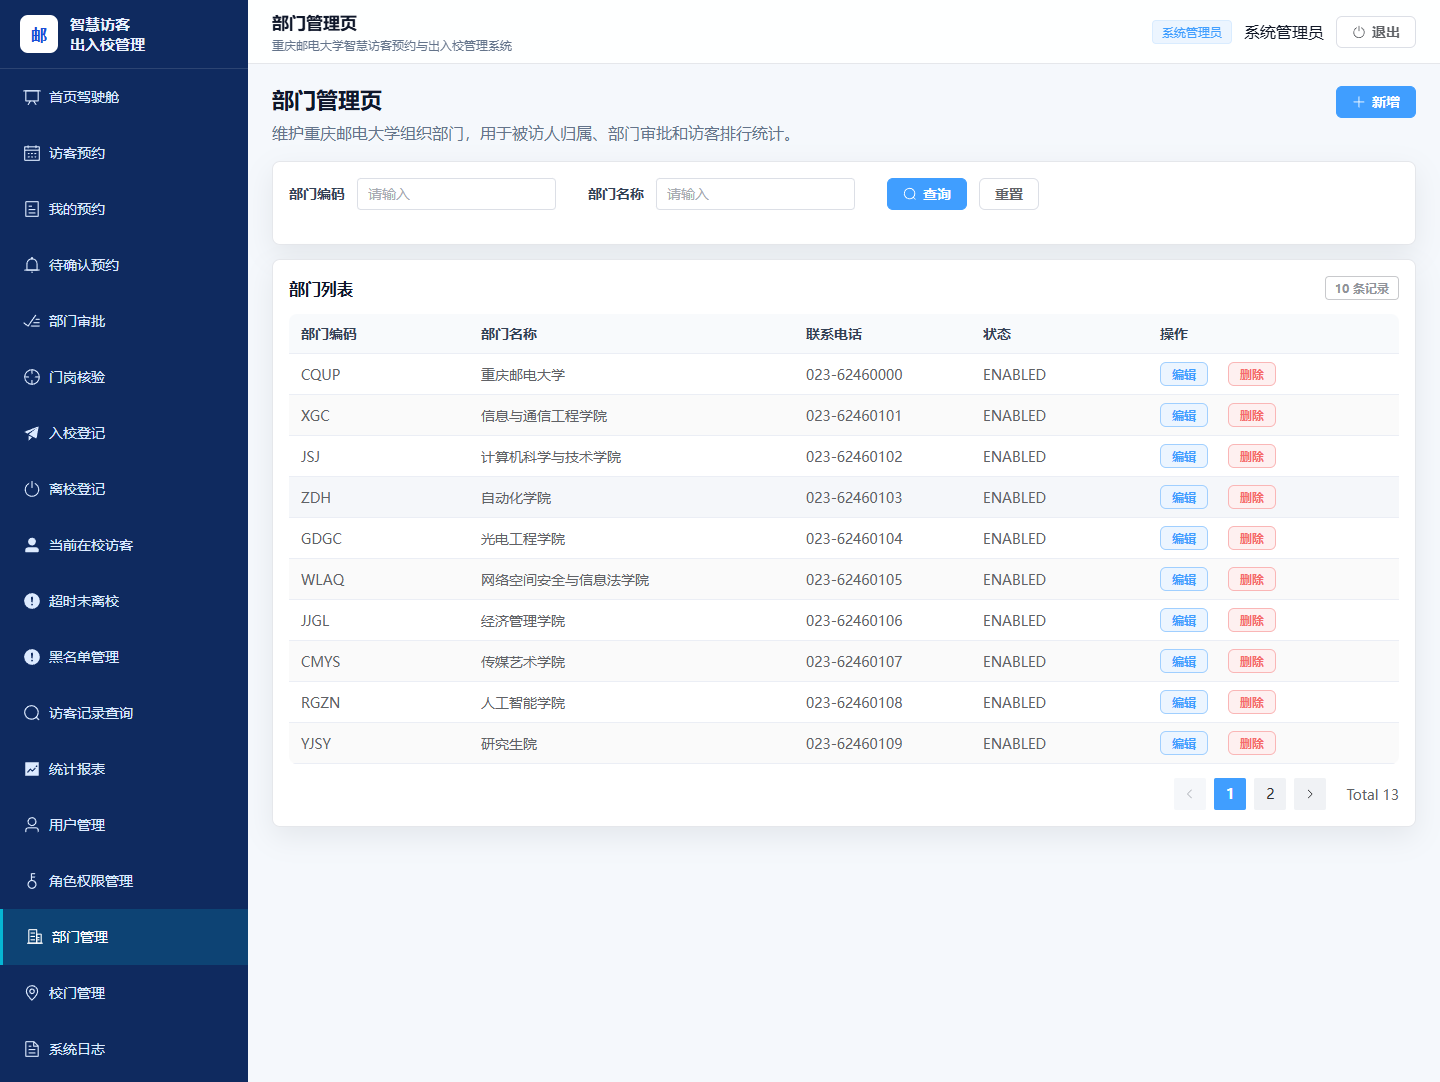
\includegraphics[width=0.92\textwidth]{figures/17_department_manage.png}

  \caption{部门管理页}

\end{figure}

展示腾飞门、北门、崇文门等校门基础数据维护。

\begin{figure}[H]

  \centering

  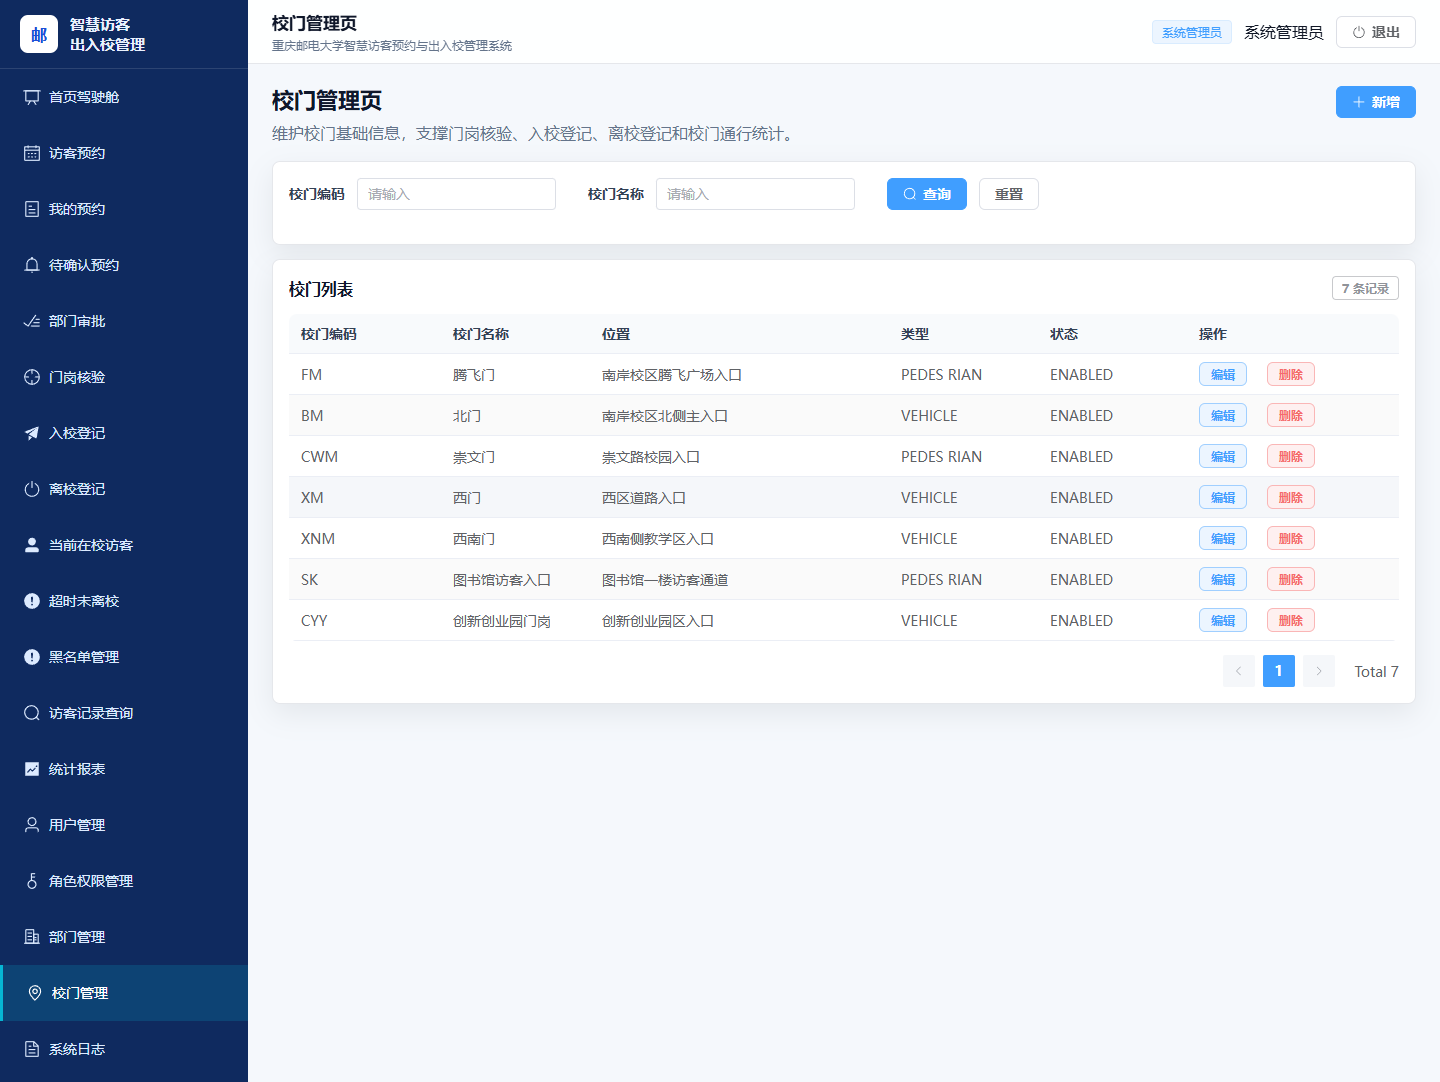
\includegraphics[width=0.92\textwidth]{figures/18_gate_manage.png}

  \caption{校门管理页}

\end{figure}

展示登录、预约、审批、出入校登记、黑名单维护和报表查询等关键操作日志。

\begin{figure}[H]

  \centering

  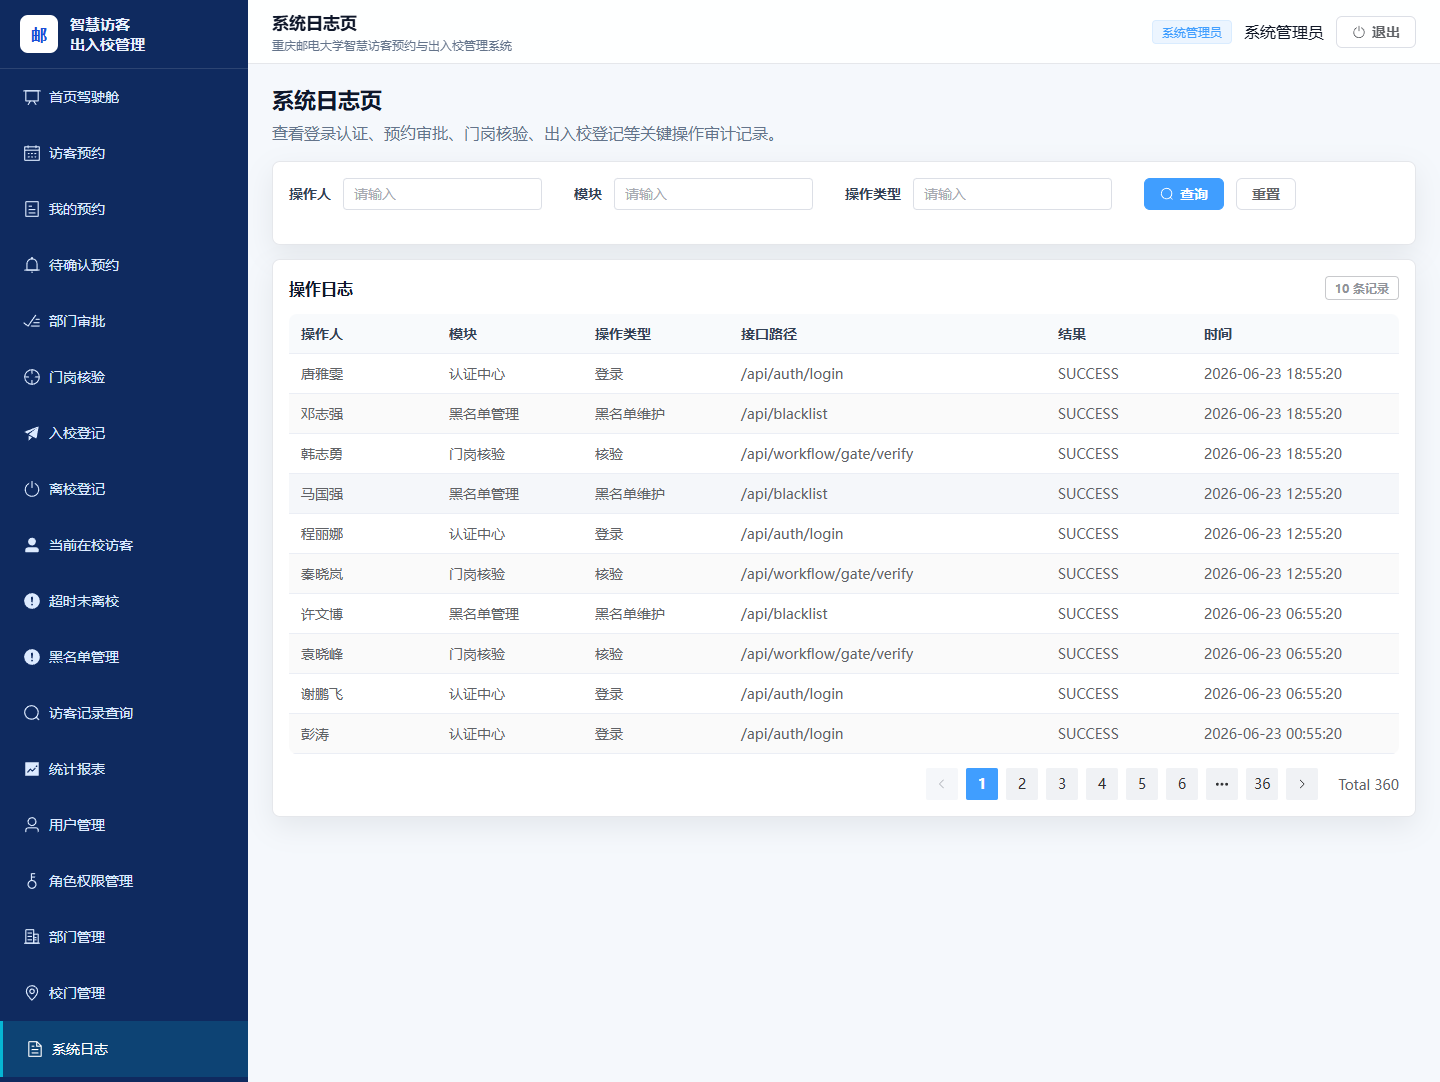
\includegraphics[width=0.92\textwidth]{figures/19_system_log.png}

  \caption{系统日志页}

\end{figure}